
%What is eels?
%Sample experimental setup
%Sample spectra
%Signal types
%usages
%pros, cons/ STEM TEM
\setcitestyle{numbers,open={[},close={]}}


The focus of this work lies on theoretical calculations from first principles, designed to provide information on materials without the need for experiment.  However, in order to verify new techniques, they must be confirmed with experiment.  To this end, this chapter will commence with an overview of experimental electron microscopy and  energy loss spectroscopy(EELS) before investigating how it is performed in the  structure of density functional theory (DFT). We will conclude with a review of the various methods used to calculate EELS theoretically.  The particularities of lithium materials will be discussed at each step of this process.  
 
\section{Electron Energy Loss Spectroscopy}

\subsection{Background}
Materials are becoming increasingly refined with properties requiring characterization of nano scale features to unlock their full potentials \cite{goldstein_electron_2003}.  At these length scales, even state of the art light microscopes lack the resolution to discern these features \cite{rust_sub-diffraction-limit_2006}.  This limitation is due to the fact that nano scale features fall well below the diffraction limit of light microscopes \cite{hecht}: 

\begin{equation}
	d = \frac{\lambda}{2n\textrm{ sin}(\theta)}
\end{equation}

Where n is the refractive index and d is the smallest distance between 2 discernible objects. For optical light ($\lambda$ = 400-800nm), it is impossible to routinely achieve the desired resolution ($\sim$ 1-50 nm) for characterization \cite{rust_sub-diffraction-limit_2006}.  Electrons however have a wavelength dictated by \cite{goldstein_electron_2003}: 
\begin{equation}
 \lambda = \frac{h}{\sqrt{2 m_0 e E}}
\end{equation}
Where $h$ is planck's constant, $m_0$, $e$ and $E$ are the rest mass, charge and energy of an electron.  In an electron microscope, electrons are accelerated to energies on the order of 1-100 keV giving them wavelengths in the range from 1-100 pm ($1\mathrm{pm}=10^{-12}$m).  Electron microscopes can therefore achieve a far lower theoretical diffraction limit  and are currently limited by the technological constraints of the electron  lenses \cite{goldstein_electron_2003}.  Because of this high resolution, electron microscopes have become a key part of investigating material microstructure \cite{inkson_2_2016}.  This dramatic increase in resolution compared to alternative methods is illustrated in Fig \ref{method_scales}. 
\begin{figure}
	\centering
	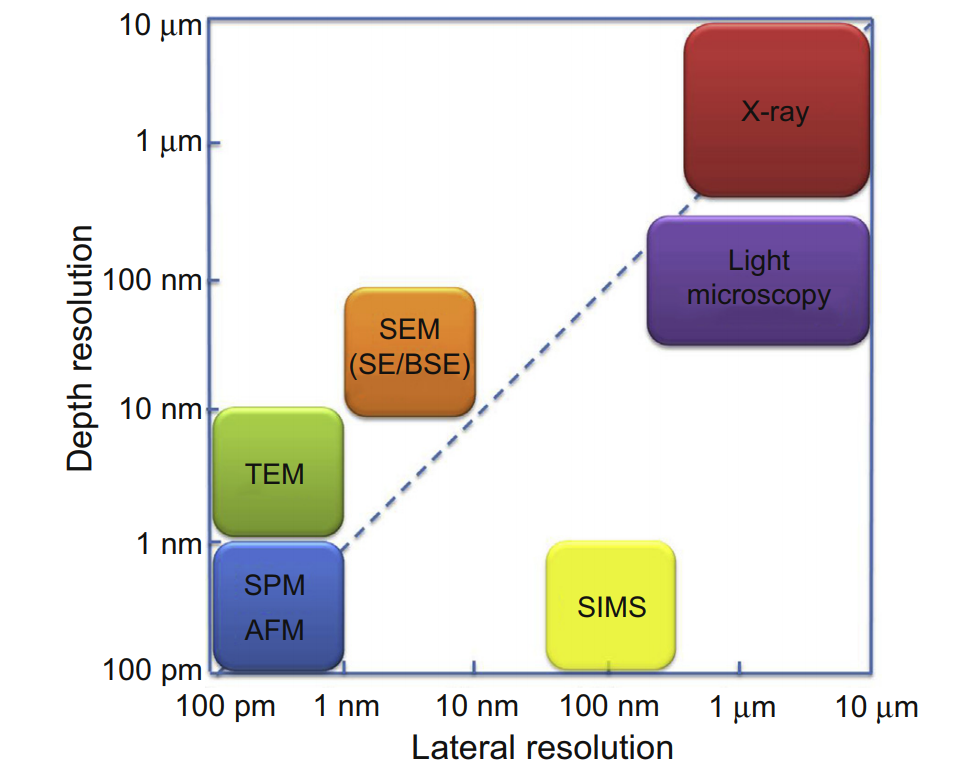
\includegraphics[scale=0.3]{method_scales}
	\caption{Resolution achievable by various techniques including Transmission and Scanning electron microscopy (TEM/SEM) and light microscopy, on a log-log scale.  Taken from Inkson, 2016 \cite{inkson_2_2016}}.
	\label{method_scales}
	
\end{figure}

In addition to the ability to image samples with high resolution, electron microscopy generates a large number of different and useful signals which can be used for both to characterize samples as well as imaging them, see Fig \ref{specimen_emmisions} \cite{williams_transmission_2008}.  A full discussion of the various techniques electron microscopes used to investigate each of these accessible signal types is beyond the scope of this work and has been well documented elsewhere \cite{goldstein_electron_2003,Egerton,williams_transmission_2008,reimer_electron_1998}.  Instead, we will focus on the relevant technique, electron energy loss spectroscopy (EELS).  EELS is an electron microscopy technique that analyzes the transmitted inelastically scattered electrons, Fig \ref{specimen_emmisions}\cite{Egerton}.  It is mainly an analytic technique, however it is also possible to perform imaging with EELS \cite{varela_stem-eels_2012}.  EELS consists of collecting electrons that have passed entirely through the sample and binning them according to how much energy each one has lost, resulting in a spectrum such as in Fig \ref{EELS_spectra}.  The mechanism of energy loss for the beam electrons is by exciting the samples electrons in a number of ways, which is reflected by the multiple different features in the spectrum \cite{Egerton}. The main features in EELS spectra are: 
\begin{figure}
	\centering
	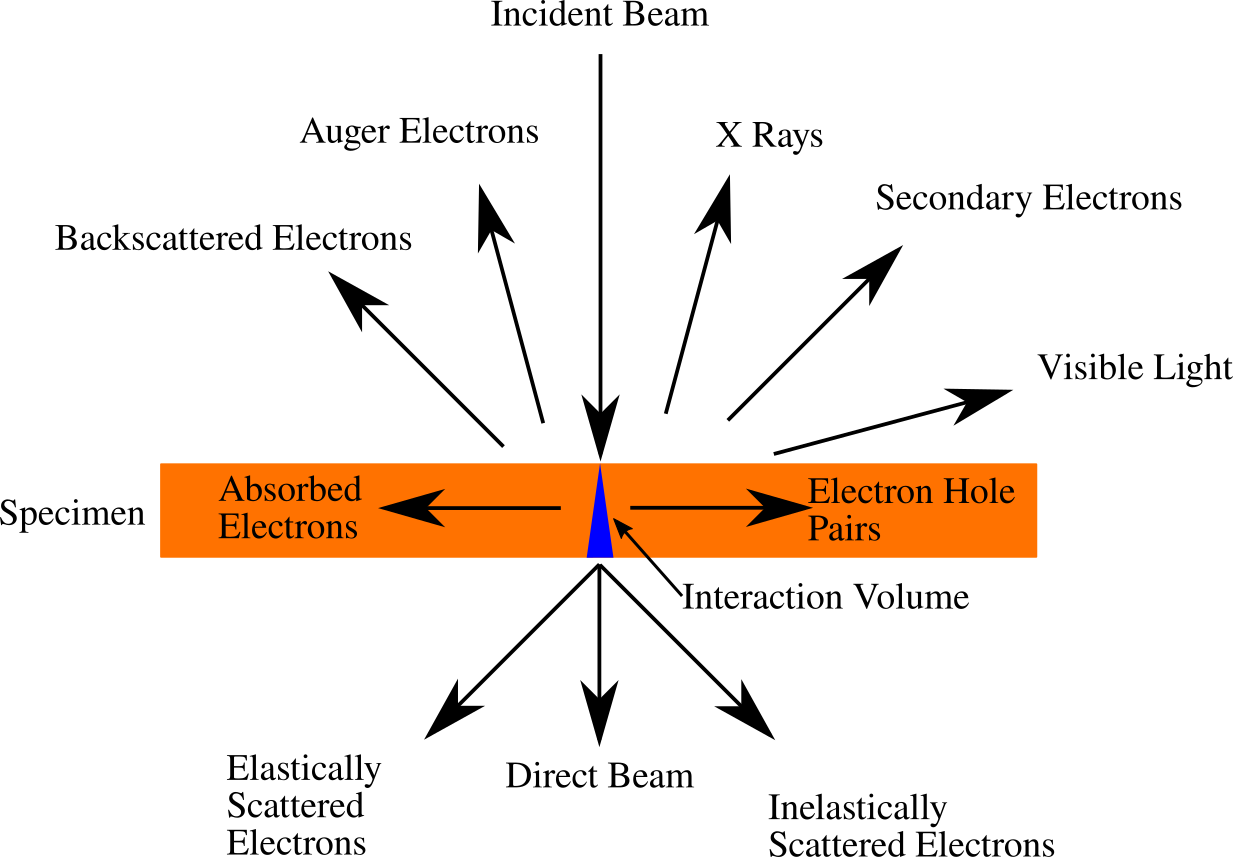
\includegraphics[scale=0.3]{specimen_emmisions.png}
	\caption{The numerous types of signals emitted when an electron beam encounters a sample in a TEM/STEM.   Redrawn from Williams and Carter \cite{williams_transmission_2008}.  }
	\label{specimen_emmisions}
\end{figure}

\begin{figure}
	\centering
	
\includegraphics[scale=0.3]{EELS_spectra.png}
	\caption{Sample EELS spectra identifying the main features, the zero loss peak, plasmon peak and ionization edges wwith fine structure.   The intensities are on a log scale, and span approximately 6 orders of magnitude between the zero loss and the ionization edges.  }
	\label{EELS_spectra}
\end{figure}

\begin{itemize}
	\item \textbf{Zero Loss Peak:} The majority of the electrons in EELS pass through the specimen without experiencing an inelastic interaction, and retain their initial energy.  The width of this peak defines the resolution of the spectrum and is due to energy spreading as the beam passes through the electron lenses \cite{colliex_illustrated_1985}.  For thin samples, zero loss peak is also the most intense feature on a spectrum \cite{Egerton}.  
	
	\item \textbf{Plasmon Peak:}  The electron beam can excite multiple atoms in the solid collectively, creating a wavelike oscillation in electron cloud of the solid \cite{Egerton}.  These ae called plasmon excitations and result in a peak appearing between 5-30eV \cite{Egerton}.  The shape and intensity of the peak is dependent on the bond strength in the material and can be used to probe properties such as thickness and surface topology \cite{malis_eels_1988,nelayah_mapping_2007}. 
	
	\item \textbf{Ionization Edges:} Beam electrons can also excite core electrons in the sample to the conduction band.  As an atom's core states are in general isolated from its surroundings, the ``edges" for each element will occur at specific energy locations, independent of sample, analogous to characteristic x-rays \cite{Egerton}. These can be used to determine sample composition \cite{Egerton}.  
	
	\item  \textbf{Background:} Beam electrons can excite loosely bound electrons close to the Fermi level into the unoccupied conduction band.  Due to the large number of possible transitions and the fact that high energy events are less favourable, this results in a smoothly decaying background \cite{Egerton}.

	
\end{itemize}

%The probability of each event depends on a number of factors.   Foremost amongst these is that the higher the energy of an event, the less likely it is to occur (CHECK!!!). This is highly dramatic as can be seen by the N orders of magnitude required to show all of these features.  

Another key factor that needs consideration, is that in order for meaningful data to be extracted from a spectra, the number of electrons that experience multiple inelastic events must be minimized \cite{Egerton}.  If not, duplicate plasmon peaks will appear in the spectra, and because of their relatively high intensity, the weaker ionization edges will become drowned out by the background, see Fig \ref{multiple_plasmons}. As well, any electron that experiences an ionization event will likely also experience some form of plasmon interaction, further smearing any ionization edges in thicker samples.  

\begin{figure}
	\centering
	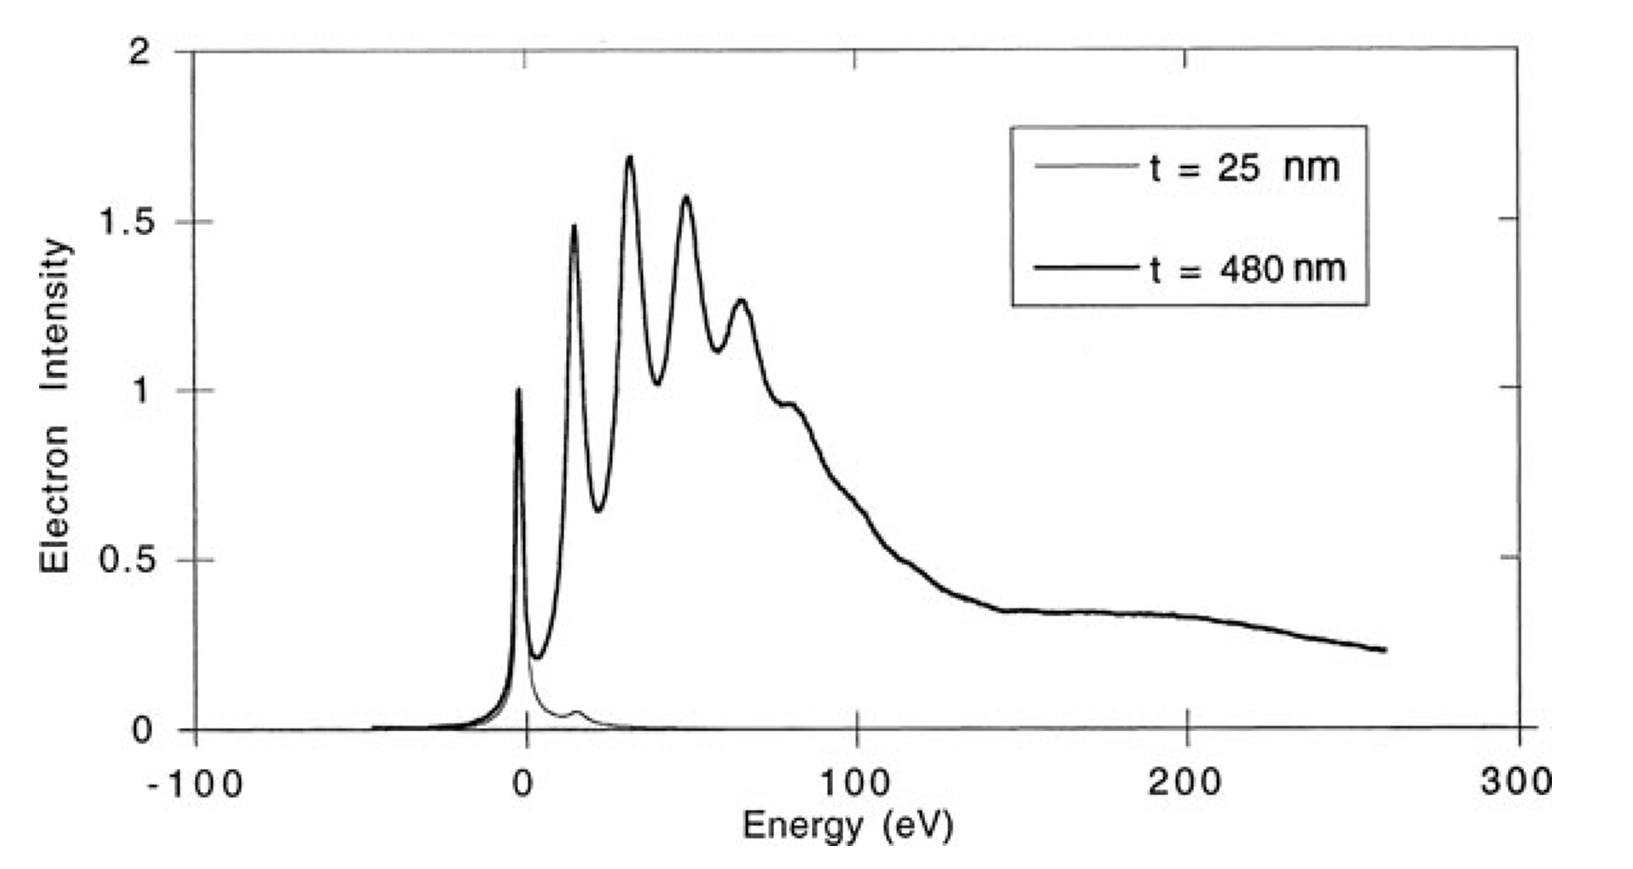
\includegraphics[scale=0.2]{multiple_plasmons.png}
	\caption{Two spectra demonstrating the importance of thin samples and single scattering events. In the thicker sample, the majority of beam electrons experience one or multiple plasmon excitations, resulting in multiple evenly spaced plasmon peaks with larger intensity than the zero loss.  The higher background from the plasmon peaks and the thicker sample drown out any structure due to ionization edges \cite{Egerton}. Image taken from Egerton, 2011 \cite{Egerton}}
	\label{multiple_plasmons}
\end{figure}



\subsubsection{Near Edge Structure}
Unlike x-ray edges in EDS which have distinct, simple shapes, higher energy resolution in EELS reveals additional features in the ionization edges extending up 50 eV beyond the onset of the edge \cite{Egerton}.   These features are a reflection of the unoccupied states in the conduction band that represent the final states of sample electrons excited by the beam.  The band structure of the conduction band is largely dependent on the local bonds of the atom in question.  Because of this, ELNES can be used to investigate the local environment of each element.  This can be used to distinguish different crystal structures of the same element such as carbon in graphite vs diamond, see Fig \ref{carbon-k-edge} \cite{hamon_elnes_2004}.  ELNES is also sensitive to impurities that would effect the band structure.  

\begin{figure}
	\centering
	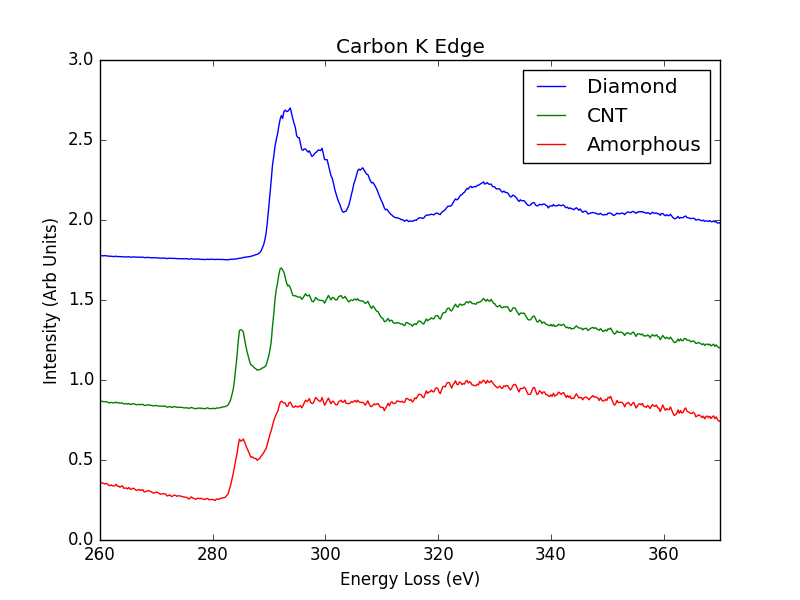
\includegraphics[scale=0.5]{Carbon_k_edges}
	\caption{Carbon K edge taken at 30keV at McGill. The different crystal structures (amorphous, diamond and carbon nanotube) result in distinctly different ELNES which can be used for identification.   }
	\label{carbon-k-edge}
\end{figure}


\subsection{EELS in Experiment}

In order to collect EELS spectra, electrons must pass entirely through the sample, making EELS a technique for transmission electron microscopes (TEM's)\cite{Egerton}. In order to collect these transmitted electrons, a magnetic field prism is placed below the specimen and redirects the electrons into a detector, Fig \ref{prism}.  Inside the magnetic prism, there is a $\mathrm{\textbf{B}}$ field perpendicular to the beam direction and the transmitted electrons are exposed to a Lorentz force: 


\begin{equation}
	\textbf{F}_B = q (\textbf{v} \times \textbf{B})
\end{equation}

As the force varies according to the velocity of the electrons, the magnetic prism  separates the electrons according to their energy: 

\begin{gather}
\textbf{F}_B = e (\textbf{v} \times \textbf{B}) =  \frac{m \textbf{v}^2}{\textbf{r}} = \textbf{F}_c \\
 r =  \frac{mv}{eB} = \frac{\sqrt{2mE}}{eB}
\end{gather}

\begin{figure}
 \centering
 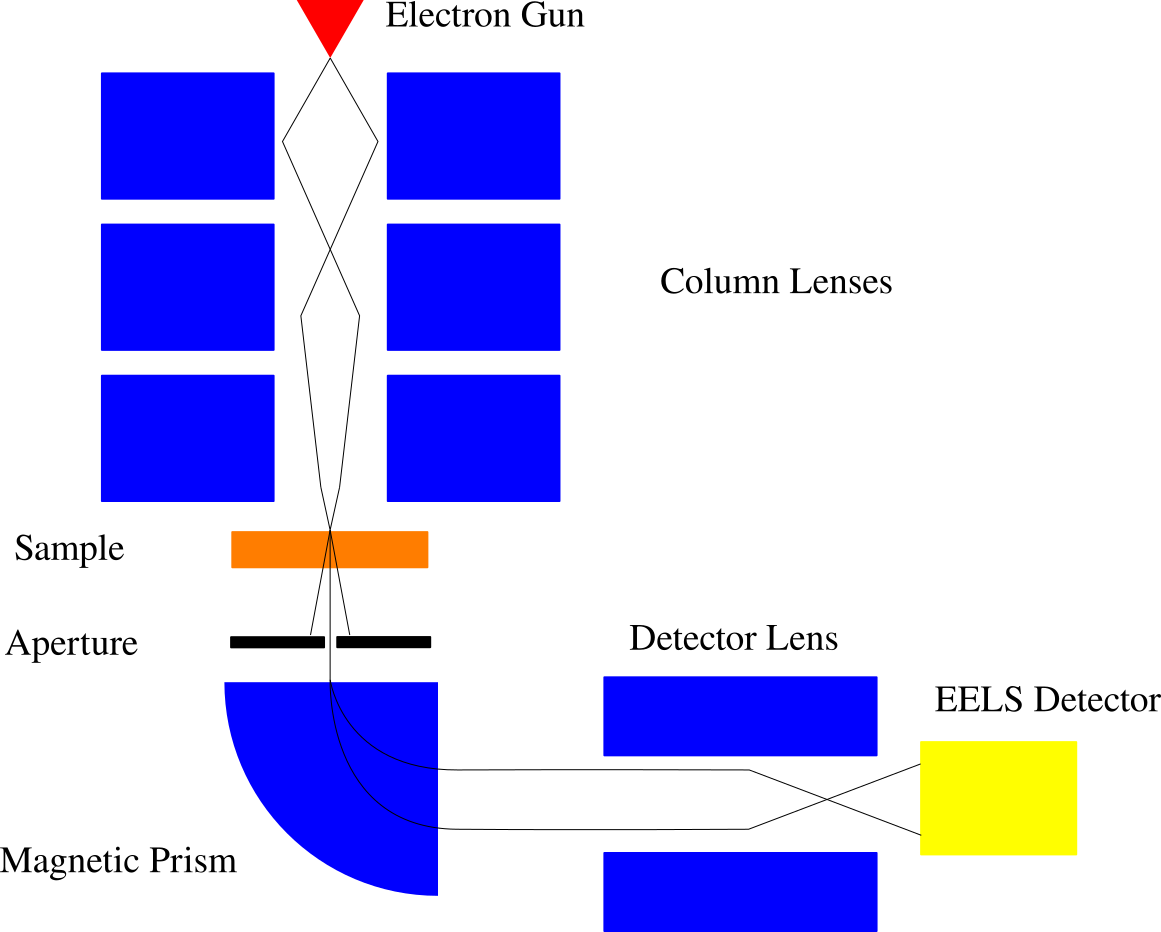
\includegraphics[scale=0.4]{Expt_setup.png}
 \caption{Experimental EELS setup, with the various magnetic lenses depicted in blue.  }
 \label{prism}
 
\end{figure}

Where e is the charge of an electron and E is the energy of each electron after passing through the sample.  By mapping each location on the detector to a corresponding energy loss value the final spectra are obtained. In order to produce images, the beam is rastered over the sample and the intensities of a specific energy loss value are used to create an image. 

\subsubsection{TEM vs SEM EELS}
There are two main types of electron microscopy, scanning and transmission (SEM and TEM).  TEM typically operates with beam energies between 100-300 keV while SEM performs between 1-30 keV.  Each method has their own set of advantages.  TEM's operate on thin samples resulting in a minimal interaction volume, resulting in far higher energy resolution and have the ability to image individual atoms. SEM's scan the surfaces of samples and can operate on bulk specimens.  SEM is also dramatically more economical and flexible of a technique.   EELS has been conventionally performed in TEM's as it requires the beam to pass through the sample. Recent advances however have allowed EELS to be performed in an SEM.   EELS in an SEM offers the distinct advantage over TEM EELS for lithium materials as it allows operation at 30keV which minimizes the beam damage.  It is also dramatically more economical.   

\subsubsection{Lithium in EELS}
Lithium materials present a number of challenges to EELS analysis.  As the lightest alkali metal it is almost always ionized and highly mobile. Additionally, lithium ion battery materials are in general insulators with band gaps of varying sizes. These features make lithium materials highly sensitive to electron beam damage.  This damage results from the charge buildup when an electron beam passes through a sample.  In electron conductive samples (eg. metals), this charge can be dissipated to a certain extent, however in materials with a band gap (eg. insulators, battery cathodes), this charge can displace the charged and mobile lithium ions and break down the crystal structure.  Lithium's high mobility also make them vulnerable to knock on damage.  This effect occurs when an electron interacts inelastically with an atom's nucleus and transfers sufficient energy to it to displace it from its lattice site.  Lithium is particularly vulnerable to this interaction because its lightweight and high mobility, meaning that it requires only a small amount of energy ($ \sim 1-5$eV) to displace it through a crystal.\\  
Lithium's only ionization edge is its K-edge is located at $\mathrm{\sim}$55eV, at the boundary of what is considered reasonable for analysis.  The low edge places it close to the plasmon decay complicating background subtraction.  This energy range also often results in overlap between the lithium K-edge and the $\mathrm{M_{2 / 3}}$ and $\mathrm{M_4}$ edges of transition metals. In particular the edges of Mn, Fe and Ni, all fall between 40-70eV.  As these elements are key components to cathode materials, they can require further steps for analysis to be possible.



\subsection{Preprocessing}

There are two key steps to be performed upon acquiring an ELNES spectra before it can be used for meaningful conclusions, background subtraction and deconvolution. 

\subsubsection{Background Subtraction} \label{bg_section}
The smooth decaying background in EELS spectra needs to be removed in order for meaningful comparison and measurements to be made on ELNES.  However, the EELS background does not decay at a fixed rate and changes based on the presence of edges and with energy \cite{new_bg}. Consequently, it is not currently possible to fit remove a single function to an entire spectrum.  Instead, the method of choice relies on fitting to a window directly before an ionization edge and refitting for each edge as needed.  The most prevalent function used for this purpose is a power law decay \cite{Egerton}: 

\begin{equation}
	I_{bg} = AE^{-r}
\end{equation}

Where E is the energy loss and A and r are fitting factors.  This method has limitations due to different regions of the spectra decaying at different rates which means a fit must be performed for every analysis \cite{verbeeck_model_2004, egerton_inelastic_1975}.  A downside of this method is the final results dependence on the size and location of the fitting window on the final output, see Fig \ref{bg_removal}.  This instability has resulted in a number of alternate models being proposed for specific cases, however, the power law method remains the most prevalent \cite{verbeeck_model_2004, riedl_extraction_2006}.  

\begin{figure}
	\centering
	\begin{subfigure}{0.45\textwidth}
		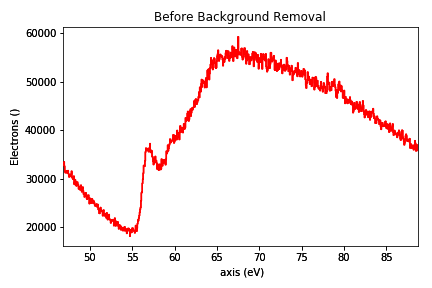
\includegraphics[scale=0.5]{full_bg.png} 
		\caption{}
		\label{full_bg}
	\end{subfigure}
	\hfill
	
	\begin{subfigure}{0.45\textwidth}
		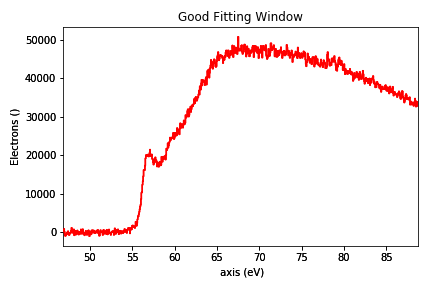
\includegraphics[scale=0.5]{good_window.png} 
		\caption{}
		\label{good_window}
	\end{subfigure}
	\begin{subfigure}{0.45\textwidth}
		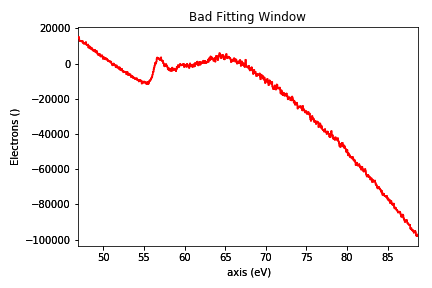
\includegraphics[scale=0.5]{bad_window.png} 
		\caption{}
		\label{bad_window}
	\end{subfigure}
	\caption{Results of power law background removal from raw spectrum (a) of metallic lithium K edge, using an appropriate (b)and inappropriate (c) window choice.}
	\label{bg_removal}
\end{figure}

\subsubsection{Deconvolution} \label{deconvolution}
Despite drastic improvements, there is still a degree of energy spread on beam electrons, typically in the range of $\sim$0.5-3eV.  This energy spread results in the observed ELNES on a spectra to be a result of a convolution between the 'actual' ELNES and the zero loss peak.  Additionally, the probability of an electron undergoing plural scattering (scattering inelastically more than once in the specimen) must also be accounted for, as the low loss region of the spectrum is also convoluted into the output spectra.  Plural scattering can best be seen in thicker samples where it results in the presence of multiple plasmon peaks, although it is present on the entire spectrum.  In order to recover the single scattering spectrum, the output must undergo deconvolution.  A number of techniques exist for this purpose.   Fourier techniques rely on describing the signal as a number of convolutions:

\begin{equation}
 	J(E) = Z(E))\ast[\delta(E) + \frac{S(E)}{I_0} +  \frac{S(E) \ast S(E)}{2! I_0}   + ...]
\end{equation}



Where J(E) is the obtained spectra, Z(E) is the zero loss peak, S(E) is the single scattering spectra, and I$_0$ is the integrated intensity of the zero loss.  The double scattering term is the convolution of the two single scattering terms, weighted by the decreased probability according to Poisson statistics.   Taking a Fourier transform of this turns all of the convolutions into products: 

\begin{equation}
	j(\nu) = z(\nu) \left(1+\frac{s(\nu)}{I_0}+   \frac{s^2(\nu)}{2! I_0}+ \frac{s^3(\nu)}{3! I_0} + ...\right)
	\label{fourier_spectra}
\end{equation} 

Which can in turn be collapsed into an exponential:

\begin{equation}
	j(\nu) = z(\nu)\mathrm{exp}[s(\nu)/I_0]
\end{equation}

This equation can then be solved for $s(\nu)$ and reverse Fourier transformed to obtain the single scattering spectra.  In order to avoid amplifying the noise in the original spectra, which is represented by high frequency terms in Fourier space, the result must be broadened by a modifier to minimize these terms.  Thus, deconvolution can only improve the energy resolution of a spectra to a certain extent.  

More recently, Bayesian methods have found success as well, in particular the Richardson-Lucy technique \cite{richardson_lucy}. This technique is based on iterative methods initially developed in astronomy and used for the deconvolution of images, including some from the Hubble space telescope \cite{hubble}.  From the same starting point, the convolution of the ideal spectra with the low loss, or point spread function:

\begin{equation}
J(E) = R(E)\ast S(E)
\end{equation}

As an EELS spectra is inherently pixilated by the CCD, at each pixel we can apply Poisson statistics to define the probability of obtaining the observed number of counts (N) \cite{richardson_lucy}:  

\begin{equation}
	P (N/N_m) = \frac{e^{-N_m}N^N_m}{N!}
\end{equation}

By iteratively varying N$_m$ and maximizing the probability, the deconvoluted spectra can be obtained.  Similar to Fourier methods however, the noise on the spectra increases with more iterations, in order to conserve information.   


\subsection{Other Experimental Techniques}
EELS is by no means the only experimental technique available for the analysis of material microstructure, nor is it even the only electron microscopy technique available for the task. Other prevalent techniques include x-ray based analysis such as x ray absorption spectroscopy and energy dispersive spectroscopy.  We will take a moment to briefly describe these methods.

\subsubsection{X Ray Absorption Spectroscopy (XAS)}
XAS operates on a similar principle to EELS.  Instead of probing the sample with an electron probe, a beam of x-rays is directed through the sample and the resulting energy losses in the output spectrum are binned as in EELS \cite{groot_high-resolution_2001}.  The difference in probe media does not effect the measured quantity which is the same as in EELS: the unoccupied density of states of the material \cite{groot_high-resolution_2001}.  Because of their similarities, parallels are often drawn between EELS and XAS when developing theories.  The largest benefit of XAS is it's superior energy resolution ($\sim$0.1 eV) when compared to EELS ($\sim$1 eV) allowing for more features in near edge structures to be identified\cite{Egerton, groot_high-resolution_2001}.  This benefit comes at a cost however, XAS needs to be performed in a synchrotron, making it far more costly and less accessible to perform than EELS


\subsubsection{Energy Dispersive Spectroscopy (EDS)}
EDS is another form of analytic spectroscopy performed in electron microscopy.   Unlike EELS and XAS which measure the unoccupied density of states, EDS measures the occupied DOS \cite{goldstein_electron_2003}.  Like EELS, EDS probes the sample with an electron beam, but then collects the emitted x-rays produced when the sample electrons return to their relaxed states following excitation.  These x-rays have the same characteristic energies as in EELS, but EDS lacks the resolution to distinguish fine structure.  As such, it is limited to providing composition information on samples.  EDS is however less strict on sample requirements as it does not require the thin samples needed by EELS and can therefore be used to analyze both bulk and microscale features in samples \cite{goldstein_electron_2003}.

\subsection{Lithium in EELS}
The focus of this work lies in application to lithium materials and a brief discussion of their experimental nature is in order. Lithium's lightweight, easily ionizable nature that make it ideal for battery applications come at the cost of making lithium remarkably sensitive to an electron beam. The highly energized charged beam of electrons used to analyze sample in a SEM/TEM inflicts a range of damage onto lithium samples including evaporation of lithium and collapse of crystal structures.  As such minimizing beam exposure is essential to performing measurements on lithium materials.  EELS is an effective means of reaching this target, as it is possible to obtain signal from the majority of ionization events and requires only a few seconds to obtain.  However, in EELS lithium presents a new challenge, the only ionization edge lies at $\sim$ 55 eV close to the background tail of the plasmon peak.  As a result, lithium EELS specimens must be made thin enough to minimize plural plasmon scattering or risk drowning out the relatively weak lithium k-edge features.  

A second range of features of lithium are its minimal interactions with x-rays.  As such a light element, lithium has a low fluorescence yield, producing a single x-ray per 10,000 ionization events.  Additionally, lithium's low Z number also results in a minimal cross section relative to interact with x-rays.  Consequently, lithium is essentially invisible to x-ray diffraction (XRD) techniques, and can only be detected on the most sensitive electron dispersive spectroscopy (EDS) systems.

These various features highlight impressive technological advances that have been necessary to even study lithium experimentally on this size scale.  They also demonstrate the need for strong theoretical support to interpret novel lithium results obtained in challenging situations.  




